% v2-acmtog-sample.tex, dated March 7 2012
% This is a sample file for ACM Transactions on Graphics
%
% Compilation using 'acmtog.cls' - version 1.2 (March 2012), Aptara Inc.
% (c) 2010 Association for Computing Machinery (ACM)
%
% Questions/Suggestions/Feedback should be addressed to => "acmtexsupport@aptaracorp.com".
% Users can also go through the FAQs available on the journal's submission webpage.
%
% Steps to compile: latex, bibtex, latex latex
%
% For tracking purposes => this is v1.2 - March 2012
\documentclass{sig-alternate} % v 2.5
% \documentclass{article}
% \usepackage{graphicx}
% --- Author Metadata here ---
%\conferenceinfo{Sample Conference}{'15 Potsdam, Germany}
%\CopyrightYear{2007} % Allows default copyright year (20XX) to be over-ridden - IF NEED BE.
%\crdata{0-12345-67-8/90/01}  % Allows default copyright data (0-89791-88-6/97/05) to be over-ridden - IF NEED BE.
% --- End of Author Metadata ---

% \bibliographystyle{abbrv}

\hyphenation{Ham-ming}

\usepackage{balance}


\def\pprw{8.5in}
\def\pprh{11in}
\special{papersize=\pprw,\pprh}
\setlength{\paperwidth}{\pprw}
\setlength{\paperheight}{\pprh}
\setlength{\pdfpagewidth}{\pprw}
\setlength{\pdfpageheight}{\pprh}

\begin{document}

\normalsize

\title{Key Provisioning for the Internet of Things via Light}

\numberofauthors{5}

\author{
\alignauthor
Cornelius Bock
%
\alignauthor
Daniel Werner
%
\alignauthor
Felix Wolff
%
\and
\texttt{\{cornelius.bock|daniel.werner|felix.wolff\}@student.hpi.de} \\ \\
\and
\alignauthor
Prof. Dr. Christoph Meinel\\
    \affaddr{\textit{Supervisor}}
%
\alignauthor
Konrad-Felix Krentz\\
    \affaddr{\textit{Supervisor}}
}
\toappear{}
\maketitle

The rise of the Internet of Things (IoT) is associated with an enormous increase in every-day devices that get connected to the Internet.
In order to avoid privacy issues and security threats those devices have to communicate securely using state-of-the-art encryption techniques.
However, these techniques often rely on predistributed keying material.
The secure and user-friendly provisioning of the initial keying material \textit{before} securing techniques are operational remains a major problem.
We propose a secure method for provisioning IoT-devices with keying material via light.
The transmission can be executed using an off-the-shelf smartphone and does not require any technical expertise.


Our method mainly targets private users without technical background.
As visible in Figure~\ref{fig:overview}, the user utilizes a smartphone application to enter, encode and emit keying material using the flashlight of the phone.
The mote receives the message via a light sensor and reconstructs the keying material.
After successful transmission and verification, the mote saves the keying material permanently.
On subsequent reboots, it is read from memory and immediately usable without any further action required.

\begin{figure}[t]
	\centering
	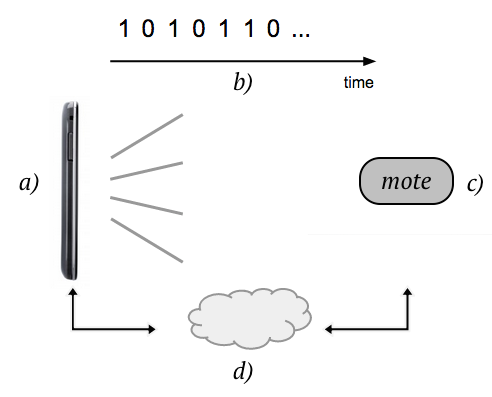
\includegraphics[scale=.65]{images/overview.png}
	\caption{Transmission of keying material with light: \textbf{a)} enter keying material and parameters on a smartphone, \textbf{b)} transmit them via light to the mote, \textbf{c)} persist keying material and parameters, \textbf{d)} communicate securely via the public Internet }
	\label{fig:overview}
\end{figure}
There are several advantages of this method.
Light sensors are smaller and less misusable than jacks.
The physics of light is well understood by non-technical people, in contrast to radio waves.
Thus, leaking of the wirelessly sent secrets is less likely.
Moreover, multiple devices could be initialized concurrently by just placing them next to each other.

We implemented a prototype for an Android smartphone and a mote running the Contiki OS.
Contiki is an open source, state-of-the-art operating system for IoT devices.
We also tested techniques to make the transmission reliable by using error detection and correcting codes and examined their usefulness with regard to data overhead and transmisison speed.
Besides, we investigated the fastest transmission speed while maintaining a high chance of correctness.
Depending on the smartphone, transmission rates between 32 and 64 bits/s are within reach.
With regard to 128 bit keys, those rates are definitely acceptable for a first prototype.
However performance varies a lot between different phone models.
We did not find a general reason for the performance differences yet.
More time needs to be invested in this topic.
Furthermore, future work should target the scaling of the presented method to initialize several motes at once.
This is a realistic scenario regarding IoT networks, where motes encrypt their communication using predistributed secret keys.
Also, one should conduct a user study to prove the usability of the prototype for users without strong technical background.

\end{document}
